% This file was created with matplot2tikz v0.5.1.
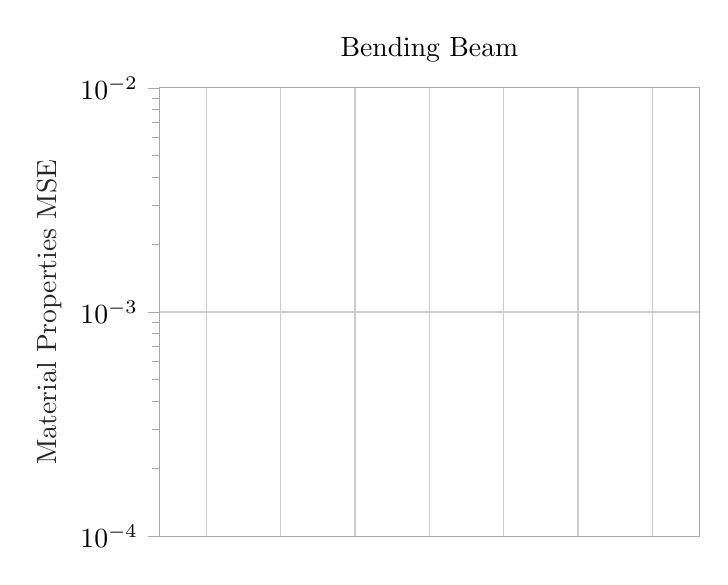
\begin{tikzpicture}

\definecolor{darkgray}{RGB}{169,169,169}
\definecolor{darkorange25512714}{RGB}{255,127,14}
\definecolor{darkslategray38}{RGB}{38,38,38}
\definecolor{darkturquoise23190207}{RGB}{23,190,207}
\definecolor{gray127}{RGB}{127,127,127}
\definecolor{lightgray204}{RGB}{204,204,204}
\definecolor{mediumpurple148103189}{RGB}{148,103,189}
\definecolor{orchid227119194}{RGB}{227,119,194}
\definecolor{sienna1408675}{RGB}{140,86,75}
\definecolor{steelblue31119180}{RGB}{31,119,180}
\definecolor{steelblue76114176}{RGB}{76,114,176}

\begin{axis}[
axis line style={darkgray},
log basis y={10},
tick align=outside,
title={Bending Beam},
x grid style={lightgray204},
xmajorgrids,
xmajorticks=false,
xmin=-0.63, xmax=6.63,
xtick style={color=darkslategray38},
xtick={0,1,2,3,4,5,6},
xticklabel style={rotate=45.0,anchor=east},
xticklabels={
  PEACH Encoder (ours),
  Mesh-based Encoder,
  No Context Encoding,
  MGN,
  MGN Oracle,
  GNN Encoder,
  PSTNet Encoder
},
y grid style={lightgray204},
ylabel=\textcolor{darkslategray38}{Material Properties MSE},
ymajorgrids,
ymin=0.0001, ymax=0.01,
ymode=log,
ytick pos=left,
ytick style={color=darkgray}
]
\draw[draw=white,fill=steelblue31119180] (axis cs:-0.3,0) rectangle (axis cs:0.3,0.201905166900158);
\draw[draw=white,fill=darkturquoise23190207] (axis cs:0.7,0) rectangle (axis cs:1.3,0.261850817298889);
\draw[draw=white,fill=gray127] (axis cs:1.7,0) rectangle (axis cs:2.3,0);
\draw[draw=white,fill=darkorange25512714] (axis cs:2.7,0) rectangle (axis cs:3.3,2.62958733568192);
\draw[draw=white,fill=mediumpurple148103189] (axis cs:3.7,0) rectangle (axis cs:4.3,2.62958733568192);
\draw[draw=white,fill=sienna1408675] (axis cs:4.7,0) rectangle (axis cs:5.3,0.824786586856842);
\draw[draw=white,fill=orchid227119194] (axis cs:5.7,0) rectangle (axis cs:6.3,2.74944473633766);
\draw [draw=black, semithick] (axis cs:0,0.183820147067308) -- (axis cs:0,0.218326382339001);
\draw [draw=black, semithick] (axis cs:-0.25,0.183820147067308) -- (axis cs:0.25,0.183820147067308);
\draw [draw=black, semithick] (axis cs:-0.25,0.218326382339001) -- (axis cs:0.25,0.218326382339001);

\draw [draw=black, semithick] (axis cs:1,0.225880924612284) -- (axis cs:1,0.323451224714518);
\draw [draw=black, semithick] (axis cs:0.75,0.225880924612284) -- (axis cs:1.25,0.225880924612284);
\draw [draw=black, semithick] (axis cs:0.75,0.323451224714518) -- (axis cs:1.25,0.323451224714518);

\draw [draw=black, semithick] (axis cs:2,0) -- (axis cs:2,0);
\draw [draw=black, semithick] (axis cs:1.75,0) -- (axis cs:2.25,0);
\draw [draw=black, semithick] (axis cs:1.75,0) -- (axis cs:2.25,0);

\draw [draw=black, semithick] (axis cs:3,2.55671906471252) -- (axis cs:3,2.687067091465);
\draw [draw=black, semithick] (axis cs:2.75,2.55671906471252) -- (axis cs:3.25,2.55671906471252);
\draw [draw=black, semithick] (axis cs:2.75,2.687067091465) -- (axis cs:3.25,2.687067091465);

\draw [draw=black, semithick] (axis cs:4,2.55671906471252) -- (axis cs:4,2.687067091465);
\draw [draw=black, semithick] (axis cs:3.75,2.55671906471252) -- (axis cs:4.25,2.55671906471252);
\draw [draw=black, semithick] (axis cs:3.75,2.687067091465) -- (axis cs:4.25,2.687067091465);

\draw [draw=black, semithick] (axis cs:5,0.666586965322495) -- (axis cs:5,0.98278620839119);
\draw [draw=black, semithick] (axis cs:4.75,0.666586965322495) -- (axis cs:5.25,0.666586965322495);
\draw [draw=black, semithick] (axis cs:4.75,0.98278620839119) -- (axis cs:5.25,0.98278620839119);

\draw [draw=black, semithick] (axis cs:6,1.3828150331974) -- (axis cs:6,4.21560209989548);
\draw [draw=black, semithick] (axis cs:5.75,1.3828150331974) -- (axis cs:6.25,1.3828150331974);
\draw [draw=black, semithick] (axis cs:5.75,4.21560209989548) -- (axis cs:6.25,4.21560209989548);

\end{axis}

\end{tikzpicture}
